\documentclass[aspectratio=169,10pt]{beamer}
\usetheme{default}
\usecolortheme{seahorse}
\usepackage[utf8]{inputenc}
\usepackage[T1]{fontenc}
\usepackage{lmodern}
\usepackage{graphicx}
\usepackage{booktabs}
\usepackage{amsmath}
\usepackage{xcolor}
\usepackage{tikz}

\graphicspath{{../figures/}}
\setbeamertemplate{navigation symbols}{}
\setbeamertemplate{footline}[frame number]
\setbeamerfont{frametitle}{size=\large}
\setbeamercolor{frametitle}{fg=blue!35!black}
\setbeamercolor{structure}{fg=blue!35!black}
\newcommand{\ns}{\,\mathrm{ns}}
\newcommand{\hl}[1]{\textcolor{orange!75!black}{\textbf{#1}}}
\newcommand{\gd}[1]{\textcolor{green!35!black}{\textbf{#1}}}
\newcommand{\ntof}{n\_TOF}

% TikZ diagrams for the DREAM <-> n_TOF matching calibration.
% Defined as macros so the same source can be dropped into the slides and into
% any other document. Requires: tikz + libraries arrows, positioning,
% shapes.geometric, fit, backgrounds, calc (all present in TeX Live 2023 base).

\usetikzlibrary{arrows,positioning,shapes.geometric,fit,backgrounds,calc}

\definecolor{stagecol}{RGB}{31,90,150}
\definecolor{incol}{RGB}{110,110,110}
\definecolor{outcol}{RGB}{20,110,60}
\definecolor{ntofcol}{RGB}{225,238,250}
\definecolor{dreamcol}{RGB}{252,238,225}

\tikzset{
  stage/.style   = {rectangle, rounded corners=2pt, draw=stagecol, very thick,
                    fill=stagecol!8, align=center, inner sep=4pt,
                    text width=#1, font=\scriptsize},
  input/.style   = {align=center, font=\tiny\itshape, text=incol,
                    text width=2.55cm},
  deliver/.style = {rectangle, rounded corners=1pt, draw=outcol!60,
                    fill=outcol!7, align=center, font=\tiny, text=outcol!60!black,
                    inner sep=3pt, text width=2.55cm},
  flow/.style    = {-latex, very thick, draw=stagecol!70},
  thin flow/.style = {-latex, thick, draw=incol!70},
  grouplab/.style = {font=\scriptsize\bfseries, text=#1},
  box/.style     = {rectangle, rounded corners=2pt, draw=black!45, thick,
                    fill=black!3, align=center, inner sep=4pt,
                    text width=#1, font=\scriptsize},
}

% ------------------------------------------------------------------
% [1] The calibration chain: inside n_TOF first, then DREAM onto it.
% ------------------------------------------------------------------
\newcommand{\calibchaindiagram}{%
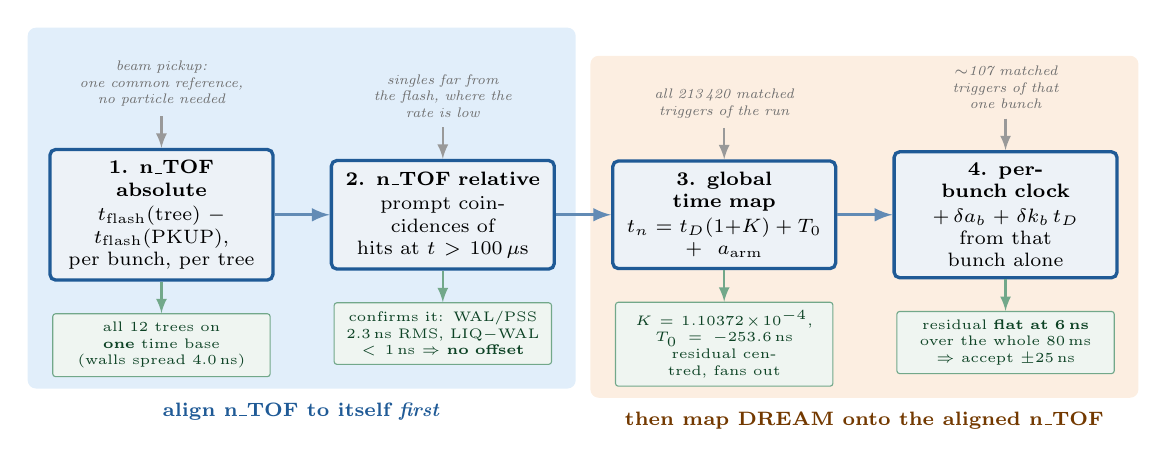
\begin{tikzpicture}[node distance=3.2mm]

  \node[stage=2.55cm] (s1)
       {\textbf{1. n\_TOF absolute}\\[1pt]
        $t_{\rm flash}({\rm tree})-t_{\rm flash}({\rm PKUP})$,\\ per bunch, per tree};
  \node[stage=2.55cm, right=7mm of s1] (s2)
       {\textbf{2. n\_TOF relative}\\[1pt]
        prompt coincidences of\\ hits at $t>100\,\mu$s};
  \node[stage=2.55cm, right=7mm of s2] (s3)
       {\textbf{3. global time map}\\[1pt]
        $t_{n}=t_{D}(1{+}K)+T_0$\\ $+\;a_{\rm arm}$};
  \node[stage=2.55cm, right=7mm of s3] (s4)
       {\textbf{4. per-bunch clock}\\[1pt]
        $+\,\delta a_b + \delta k_b\,t_{D}$\\ from that bunch alone};

  \foreach \a/\b in {s1/s2, s2/s3, s3/s4} \draw[flow] (\a) -- (\b);

  \node[input, above=4mm of s1] (i1) {beam pickup:\\ one common reference,\\ no particle needed};
  \node[input, above=4mm of s2] (i2) {singles far from\\ the flash, where the\\ rate is low};
  \node[input, above=4mm of s3] (i3) {all 213\,420 matched\\ triggers of the run};
  \node[input, above=4mm of s4] (i4) {$\sim$107 matched\\ triggers of that\\ one bunch};
  \foreach \a/\b in {i1/s1, i2/s2, i3/s3, i4/s4} \draw[thin flow] (\a) -- (\b);

  \node[deliver, below=4mm of s1] (o1)
       {all 12 trees on\\ \textbf{one} time base\\ (walls spread 4.0\,ns)};
  \node[deliver, below=4mm of s2] (o2)
       {confirms it: WAL/PSS\\ 2.3\,ns RMS, LIQ$-$WAL\\ $<1$\,ns $\Rightarrow$ \textbf{no offset}};
  \node[deliver, below=4mm of s3] (o3)
       {$K=1.10372\!\times\!10^{-4}$,\\ $T_0=-253.6$\,ns\\ residual centred, fans out};
  \node[deliver, below=4mm of s4] (o4)
       {residual \textbf{flat at 6\,ns}\\ over the whole 80\,ms\\ $\Rightarrow$ accept $\pm25$\,ns};
  \foreach \a/\b in {s1/o1, s2/o2, s3/o3, s4/o4} \draw[thin flow, draw=outcol!60] (\a) -- (\b);

  \begin{scope}[on background layer]
    \node[fit=(i1)(o2), rounded corners=3pt, fill=ntofcol, inner sep=3mm] (g1) {};
    \node[fit=(i3)(o4), rounded corners=3pt, fill=dreamcol, inner sep=3mm] (g2) {};
  \end{scope}
  \node[grouplab=stagecol, below=0.5mm of g1.south]
       {align n\_TOF to itself \emph{first}};
  \node[grouplab=orange!45!black, below=0.5mm of g2.south]
       {then map DREAM onto the aligned n\_TOF};
\end{tikzpicture}}

% ------------------------------------------------------------------
% [2] What is actually being matched, and how the fake rate is measured.
% ------------------------------------------------------------------
\newcommand{\matchflowdiagram}{%
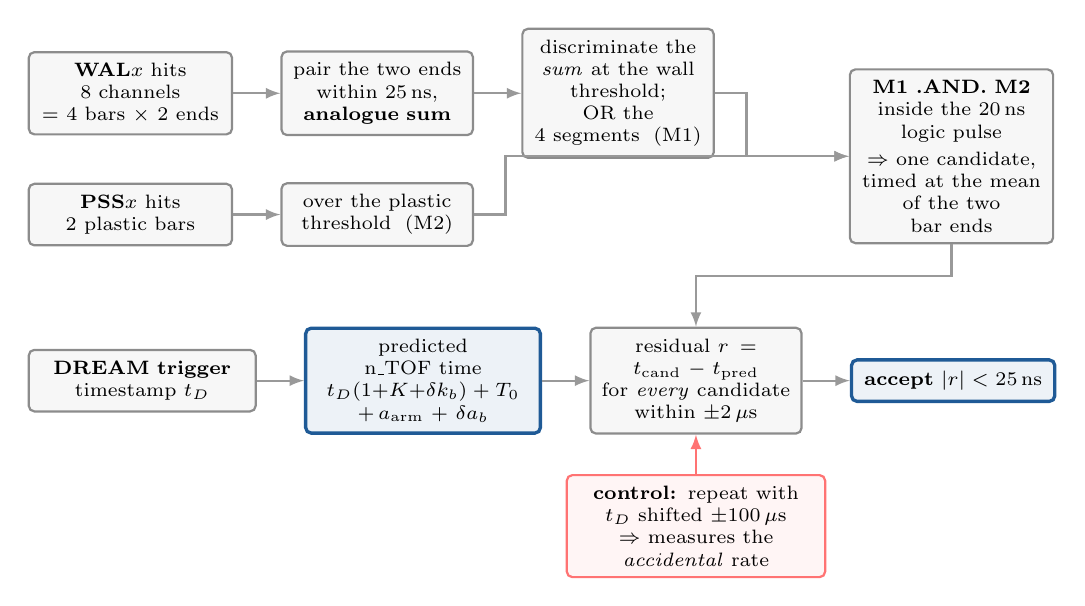
\begin{tikzpicture}[node distance=4mm]

  \node[box=2.3cm] (wal) {\textbf{WAL$x$} hits\\ 8 channels\\ $=$ 4 bars $\times$ 2 ends};
  \node[box=2.3cm, below=6mm of wal] (pss) {\textbf{PSS$x$} hits\\ 2 plastic bars};

  \node[box=2.15cm, right=6mm of wal] (sum)
       {pair the two ends\\ within 25\,ns,\\ \textbf{analogue sum}};
  \node[box=2.15cm, right=6mm of sum] (disc)
       {discriminate the\\ \emph{sum} at the wall\\ threshold; OR the\\ 4 segments \;(M1)};
  \node[box=2.15cm, right=6mm of pss] (pdisc)
       {over the plastic\\ threshold \;(M2)};

  \node[box=2.3cm, right=17mm of disc.east, yshift=-8mm] (and)
       {\textbf{M1 .AND. M2}\\ inside the 20\,ns\\ logic pulse\\[2pt]
        $\Rightarrow$ one candidate,\\ timed at the mean\\ of the two bar ends};

  \draw[thin flow] (wal) -- (sum);
  \draw[thin flow] (sum) -- (disc);
  \draw[thin flow] (pss) -- (pdisc);
  \draw[thin flow] (disc.east) -- ++(4mm,0) |- (and.west);
  \draw[thin flow] (pdisc.east) -- ++(4mm,0) |- (and.west);

  \node[box=2.6cm, below=13mm of pss.south west, anchor=north west] (dream)
       {\textbf{DREAM trigger}\\ timestamp $t_D$};
  \node[stage=2.7cm, right=6mm of dream] (map)
       {predicted n\_TOF time\\ $t_D(1{+}K{+}\delta k_b)+T_0$\\ $+\,a_{\rm arm}+\delta a_b$};
  \node[box=2.4cm, right=6mm of map] (res)
       {residual $r =$\\ $t_{\rm cand}-t_{\rm pred}$\\ for \emph{every} candidate\\ within $\pm2\,\mu$s};
  \node[stage=2.3cm, right=6mm of res] (win)
       {\textbf{accept} $|r|<25$\,ns};

  \draw[thin flow] (dream) -- (map);
  \draw[thin flow] (map) -- (res);
  \draw[thin flow] (res) -- (win);
  \draw[thin flow] (and.south) -- ++(0,-4mm) -| (res.north);

  \node[box=3.0cm, below=5mm of res.south, anchor=north, draw=red!55, fill=red!4]
       (ctl) {\textbf{control:} repeat with $t_D$ shifted $\pm100\,\mu$s\\
              $\Rightarrow$ measures the \emph{accidental} rate};
  \draw[thin flow, draw=red!55] (ctl) -- (res);
\end{tikzpicture}}


\title[DREAM$\leftrightarrow$n\_TOF matching]%
      {Matching every DREAM trigger to an \ntof{} wall\,+\,plastic coincidence}
\subtitle{The calibration, what it delivers, and why it is not fitting itself}
\author{n\_TOF X17 / DREAM analysis}
\date{2026-07-30}

\begin{document}

\begin{frame}[plain]
  \titlepage
  \begin{center}\small
  run\_79 (\texttt{stat090\_0000}\,+\,\texttt{stat090\_0001}) $\leftrightarrow$
  \ntof{} run 224572, \texttt{v12\_liqpileup} reprocessing\\
  2061 bunches, \textbf{213\,420} non-flash DREAM triggers --- the complete
  reference pair
  \end{center}
\end{frame}

% ------------------------------------------------------------------
\begin{frame}{The question, and the answer}
\begin{columns}[T]
\begin{column}{0.55\textwidth}
\textbf{Asked:}
\begin{itemize}\setlength\itemsep{0.3em}
  \item For each DREAM trigger, is there an \ntof{} SiPM-wall
        (top\,+\,bottom sum) coincident with a plastic pulse?
  \item Are the \ntof{} detectors aligned in time?
  \item What are the miss and fake rates, and how do they depend on the
        search window?
\end{itemize}
\vspace{0.5em}
\textbf{Answered:}
\begin{itemize}\setlength\itemsep{0.2em}
  \item \gd{96.0\,\%} of triggers have one. The missing 4\,\% is
        2.6\,\% plastic leg $+$ 1.4\,\% wall leg.
  \item Yes --- to a few ns everywhere, measured in situ on the file being
        analysed. The liquids need no offset at all.
  \item Once the DREAM clock is calibrated \emph{per bunch}, the match residual
        is \gd{flat at 6\,ns} over the whole 80\,ms, and \hl{$\pm25\ns$} is
        enough.
\end{itemize}
\end{column}
\begin{column}{0.43\textwidth}
\small
\begin{tabular}{lrr}
\toprule
at $|r|<25\ns$ & wall\,\&\,plastic & wall only\\
\midrule
efficiency        & \gd{95.84\,\%} & 98.30\,\%\\
accidental        & \gd{0.049\,\%} & 1.04\,\%\\
purity            & 99.998\,\%     & 99.982\,\%\\
$\geq2$ candidates& 2.46\,\%       & 5.36\,\%\\
$\geq2$ arms      & \gd{0.15\,\%}  & 3.04\,\%\\
\bottomrule
\end{tabular}
\vspace{0.6em}

\footnotesize
The accidental rate is \emph{measured, not modelled}: the identical match with
the DREAM time shifted $+100\,\mu$s. The $-100\,\mu$s control agrees
(0.062\,\%).
\vspace{0.4em}

Everything on this deck is the \textbf{whole} reference pair, and every width
quoted for the per-bunch fit is \textbf{cross-validated}.
\end{column}
\end{columns}
\end{frame}

% ------------------------------------------------------------------
\begin{frame}{What is being matched}
\begin{center}
\resizebox{!}{0.63\textheight}{\matchflowdiagram}
\end{center}
\vspace{-0.3em}
\footnotesize
The DREAM trigger was the N1081B \textbf{sector SINGLES}, so that is what is
rebuilt --- not ``any hit''. Thresholds are the values the discriminators
actually held, read from each sub-run's \texttt{n1081b\_config.json}.
The plastic requirement removes 92\,\% of the candidates
(12\,500\,$\to$\,1\,030 per bunch) for 2.6\,\% of the efficiency --- and it is
why the match is clean at 1--3\,ms, where the wall singles rate alone would
match everything by accident.
\end{frame}

% ------------------------------------------------------------------
\begin{frame}{How the calibration is built: \ntof{} to itself first, then DREAM onto it}
\begin{center}
\resizebox{0.98\textwidth}{!}{\calibchaindiagram}
\end{center}
\vspace{0.2em}
\footnotesize
The order matters. Steps 1--2 use only \ntof{} information, so they cannot be
contaminated by anything on the DREAM side; steps 3--4 then have a single,
already-consistent \ntof{} time base to map onto. Step 1 is the only one that
can compare \emph{different} detectors --- it references everything to the beam
pickup, which needs no common particle --- and step 2 is the independent check
that it worked.
\end{frame}

% ------------------------------------------------------------------
\begin{frame}{Steps 1--2: the \ntof{} detectors are aligned, measured in situ}
\begin{center}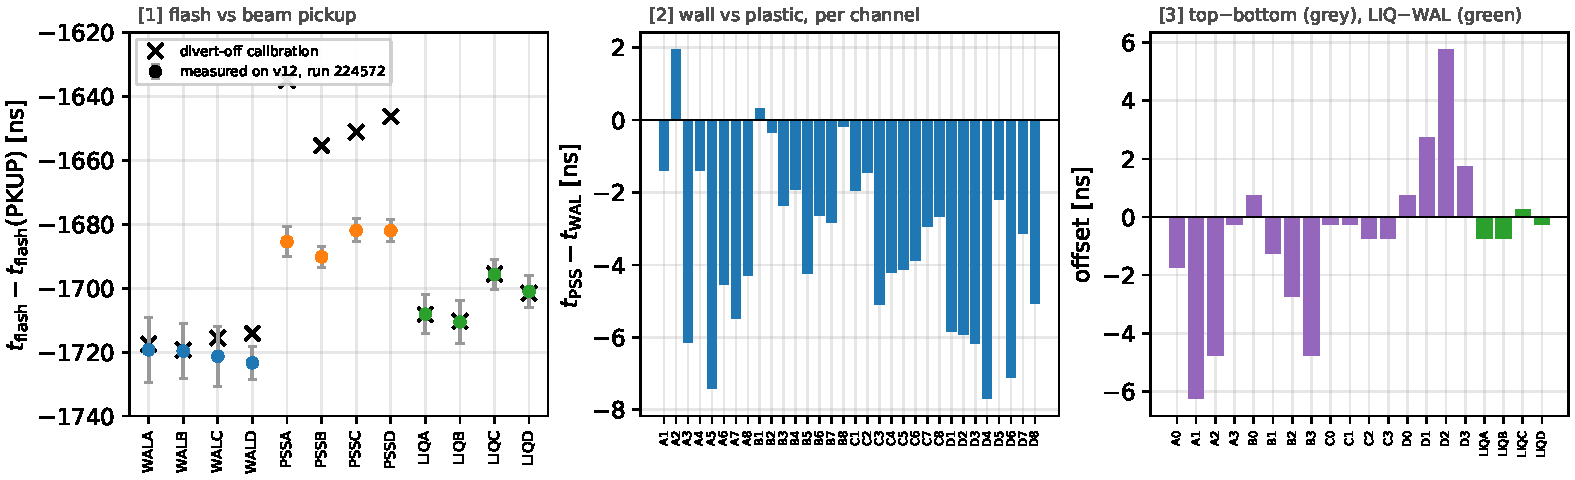
\includegraphics[width=0.93\textwidth]{fig_alignment.pdf}\end{center}
\vspace{-1.1em}
\begin{columns}[T]
\begin{column}{0.5\textwidth}\footnotesize
\textbf{[1] Absolute, vs the beam pickup.}
$t_\mathrm{flash}$(tree)$-t_\mathrm{flash}$(PKUP) per bunch.
Walls $-1719.3\ldots-1723.3\ns$ (spread \gd{4.0\,ns}).
\hl{The liquids reproduce the divert-off calibration to 0.1--0.5\,ns} --- two
independent measurements agreeing at half a nanosecond.
The plastics sit 31--50\,ns from it, exactly as \texttt{flash\_timing} warns:
take those per run.
\end{column}
\begin{column}{0.5\textwidth}\footnotesize
\textbf{[2] Wall vs plastic}, prompt coincidences of late hits ($t>100\,\mu$s):
peak $-3.8\ldots-8.8\ns$ per arm, $\sigma\simeq11\ns$;
per wall channel RMS \gd{2.3\,ns}, per plastic bar RMS 1.8\,ns.\\[0.3em]
\textbf{[3] Top vs bottom} of a bar: within \gd{$\pm6\ns$} on every segment.
\emph{Measure it on the file you analyse} --- it is a property of the pulse
reconstruction, not of the cabling.\\[0.3em]
\textbf{[4] Liquid vs wall}: $-0.8\ldots+0.2\ns$ --- \gd{aligned to under a
nanosecond}, so the liquid leg enters the merge with no offset.
\end{column}
\end{columns}
\end{frame}

% ------------------------------------------------------------------
\begin{frame}{Steps 3--4: the DREAM clock, globally and then per bunch}
\begin{center}
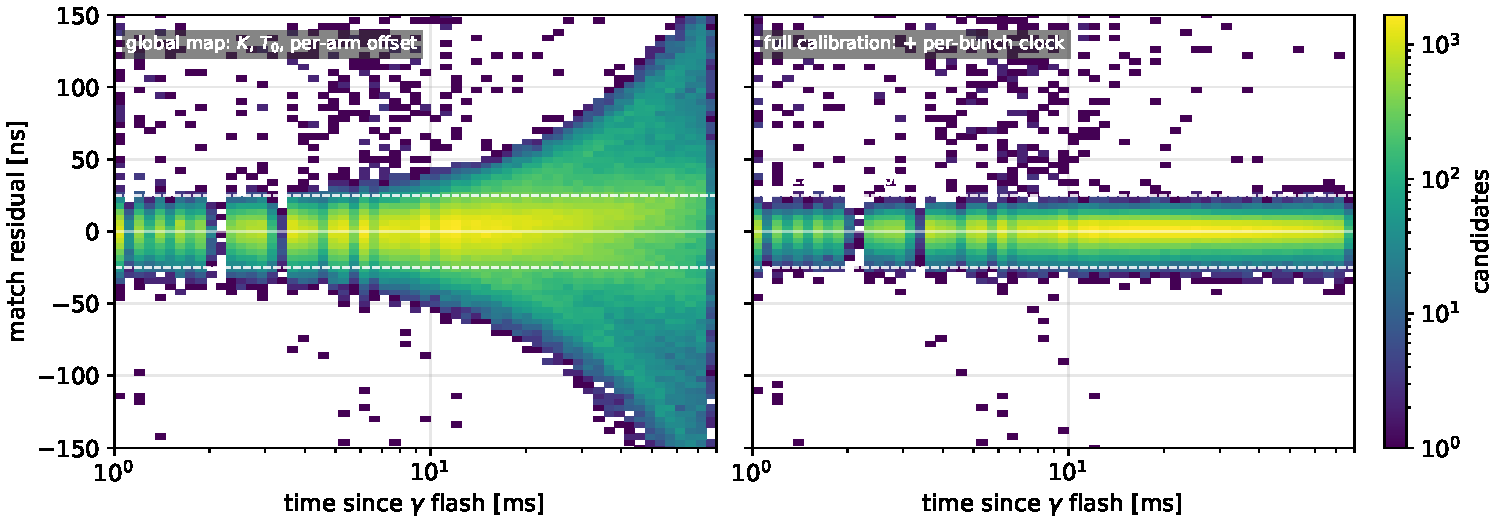
\includegraphics[width=0.95\textwidth]{fig_resid_vs_time.pdf}
\end{center}
\vspace{-0.4em}
\small
$r = t_\mathrm{\ntof} - t_\mathrm{pred}$ for every candidate within $\pm2\,\mu$s
of the prediction.\\[0.3em]
\textbf{Left, after the global map} ($K$, $T_0$, per-arm offset): centred, but
the band \hl{fans out in proportion to the time since the flash} --- $\pm9\ns$
at 1\,ms, $\pm37\ns$ at 40--80\,ms. A width proportional to elapsed time is a
\emph{rate} error, not a timing resolution.\\[0.2em]
\textbf{Right, after the per-bunch clock:} flat, and it fits inside
$\pm25\ns$ at every time.
\end{frame}

% ------------------------------------------------------------------
\begin{frame}{The DREAM timestamp clock wanders by about 1 ppm between bursts}
\begin{columns}[T]
\begin{column}{0.6\textwidth}
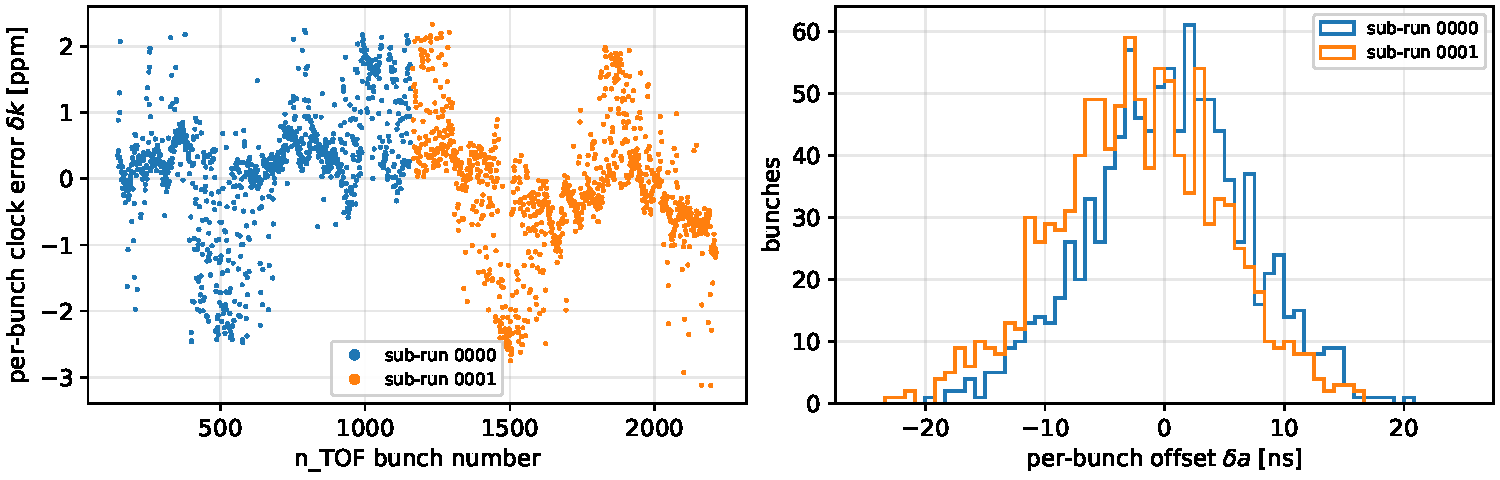
\includegraphics[width=\textwidth]{fig_perbunch.pdf}
\vspace{-0.4em}
\end{column}
\begin{column}{0.38\textwidth}\small
Fit, per bunch, from that bunch's own $\sim$107 matched triggers:
\[t_\mathrm{\ntof} = t_\mathrm{DREAM}(1{+}K{+}\delta k_b) + T_0 + a_\mathrm{arm}
  + \delta a_b\]
\begin{itemize}\setlength\itemsep{0.25em}
  \item $\delta k$: RMS \hl{0.92--0.96\,ppm}, and \emph{structured} in bunch
        number --- neighbouring bursts drift together. 1\,ppm is 60\,ns at
        60\,ms, which is the whole fan on the previous slide.
  \item $\delta a$: RMS 6.5--6.8\,ns.
  \item Fitted for \textbf{2061 of 2061} bunches.
\end{itemize}
\vspace{0.3em}
Two free parameters against $\geq$53 matched triggers per bunch, so the
correction itself is determined to \gd{0.73\,ns} --- against a 6\,ns residual.
\end{column}
\end{columns}
\end{frame}

% ------------------------------------------------------------------
\begin{frame}{Is the per-bunch fit reading back its own input? Four tests}
\begin{center}
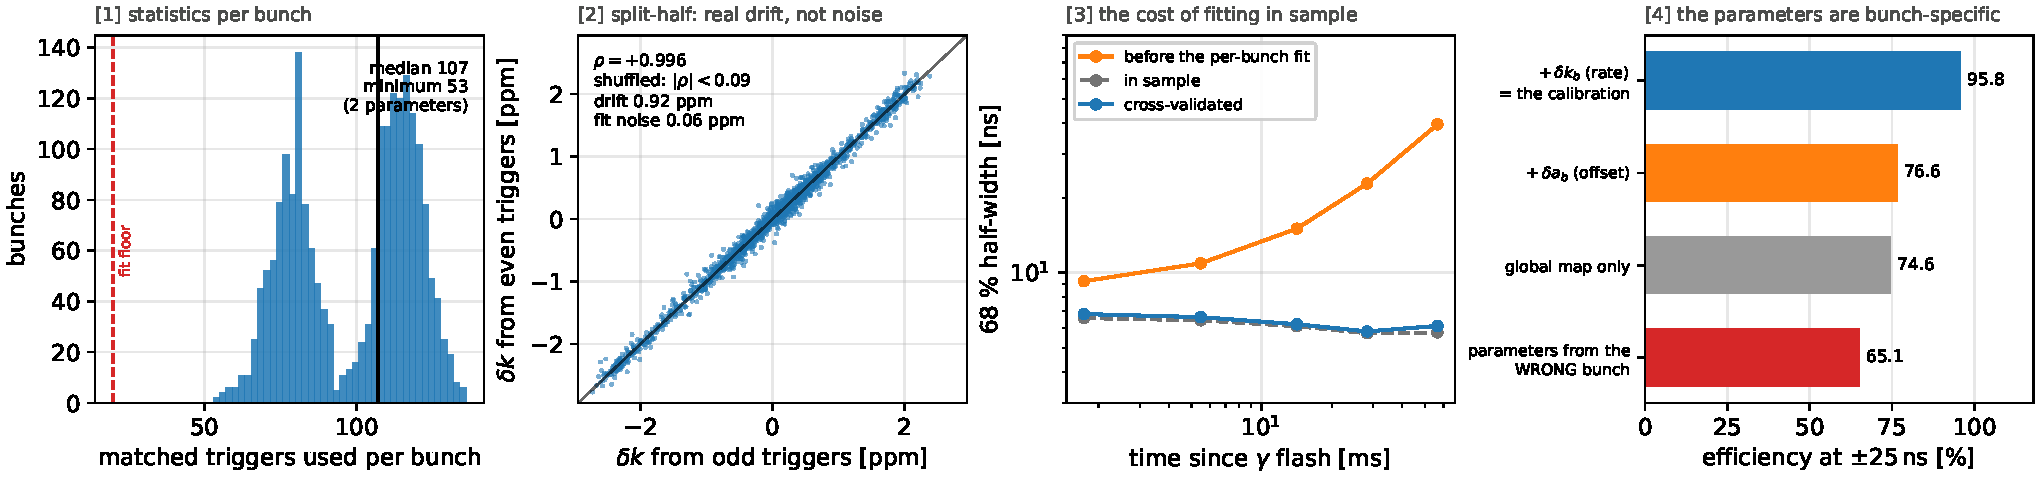
\includegraphics[width=\textwidth]{fig_bias.pdf}
\end{center}
\vspace{-0.3em}
\footnotesize
\textbf{The worry:} the clock is fitted on triggers that were matched, and then
used to match --- a 2-parameter fit that chased noise would pull the prediction
towards whatever candidate was nearest, narrowing the residual for free.
\begin{itemize}\setlength\itemsep{0.1em}
  \item[\textbf{[1]}] \textbf{107 triggers per bunch} (minimum 53) for 2
        parameters. A fit absorbs $2/N\simeq2\,\%$ of the variance, i.e.\ 1\,\%
        of a width.
  \item[\textbf{[2]}] Fit each bunch \emph{twice}, on its odd and its even
        triggers: $\rho = \gd{+0.996}$, against $|\rho|<0.09$ on 200 shuffles.
        Splitting the variance, \hl{0.92\,ppm of real drift against 0.06\,ppm of
        fit noise}.
  \item[\textbf{[3]}] In-sample vs cross-validated width: $6.5$ vs $6.8\ns$.
        \emph{That gap is the overfitting}, measured --- and everything quoted
        here is the cross-validated number.
  \item[\textbf{[4]}] Give each bunch \emph{another} bunch's parameters and the
        efficiency falls to 65\,\%, \emph{below} the uncorrected 74.6\,\%. The
        fit is carrying bunch-specific truth, not a generic shape.
\end{itemize}
\end{frame}

% ------------------------------------------------------------------
\begin{frame}{...and it cannot manufacture a match}
\begin{columns}[T]
\begin{column}{0.5\textwidth}
\textbf{The decisive test.} In a window far wider than the whole drift envelope
the correction cannot change \emph{who} is matched --- only where inside the
window they land. So if it were inventing partners, the efficiency at
$\pm500\ns$ would move:
\vspace{0.4em}

\small
\begin{tabular}{lr}
\toprule
efficiency at $\pm500\ns$ & \\
\midrule
global map only            & 96.0405\,\%\\
$+$ per-bunch clock        & 96.0405\,\%\\
\midrule
difference                 & \gd{$+0.0000$ points}\\
\bottomrule
\end{tabular}
\normalsize
\vspace{0.5em}

Identical to five decimal places. The per-bunch fit \hl{concentrates} matches;
it does not create them. What $\pm25\ns$ then buys is background rejection.
\end{column}
\begin{column}{0.48\textwidth}
\textbf{And the sample it is fitted on is clean.}
\vspace{0.4em}

The complementary test --- fit the clock on the \emph{accidental} stream and see
what it can invent --- \textbf{cannot be run}, and that is the answer: a bunch
has \hl{0.4--0.5} accidental candidates within $\pm200\ns$ of its predictions,
against the 20 the fit requires. The population the clock is fitted on is
99.95\,\% real coincidences; there is no accidental component there to fit.
\vspace{0.6em}

Consistently, applying the correction leaves the \emph{measured} accidental rate
where it was: $0.049\,\% \to 0.049\,\%$ at $\pm25\ns$, unchanged to $<0.003$
points on either sub-run.
\end{column}
\end{columns}
\end{frame}

% ------------------------------------------------------------------
\begin{frame}{The residual, and the window it allows}
\begin{center}
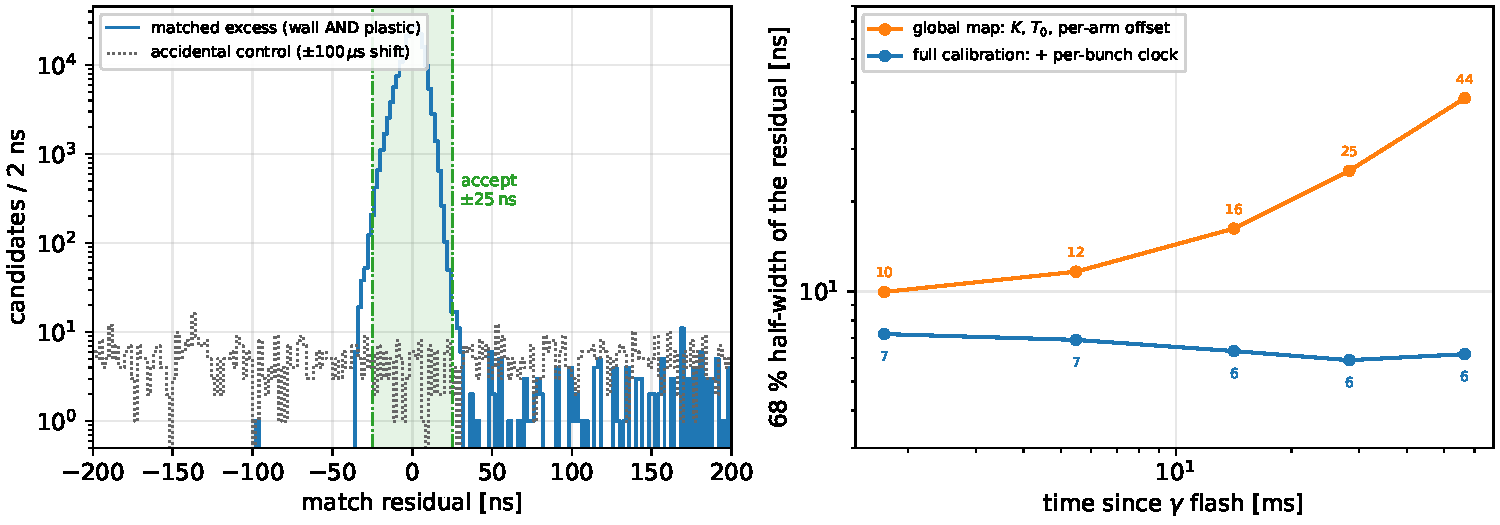
\includegraphics[width=0.92\textwidth]{fig_residuals.pdf}
\end{center}
\vspace{-0.5em}
\footnotesize
\textbf{Left:} the matched excess over the accidental control. A clean single
band --- no satellite, no tail structure. \textbf{Right:} its 68\,\% half-width
against time since the flash, before and after the per-bunch step of the
calibration: $10\to7\ns$ at 1--3\,ms and $44\to6\ns$ at 40--80\,ms, i.e.\
\gd{flat at $\simeq6\ns$ across the whole 80\,ms}. That $6\ns$ is the real
DREAM$\leftrightarrow$\ntof{} match resolution.
\end{frame}

% ------------------------------------------------------------------
\begin{frame}{Misses and fakes versus the search window}
\begin{center}
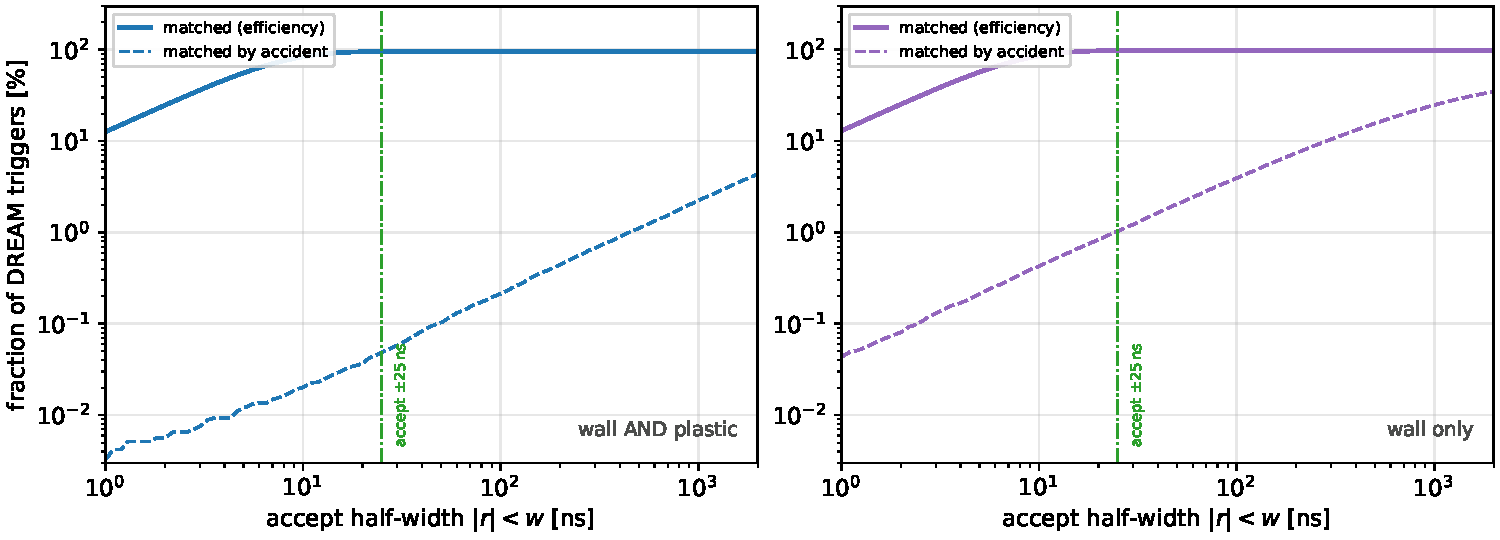
\includegraphics[width=0.97\textwidth]{fig_window_scan.pdf}
\end{center}
\vspace{-0.5em}
\small
Solid: the fraction of DREAM triggers matched. Dashed: the same with the DREAM
time shifted $+100\,\mu$s, i.e.\ the rate of matching by accident.\\[0.3em]
The accidental rate is \emph{linear} in the window width --- it is a Poisson
singles rate --- while the efficiency is flat from $\sim$25\,ns outward. Every
nanosecond of window beyond the knee is therefore pure background, bought for
nothing.
\end{frame}

% ------------------------------------------------------------------
\begin{frame}{The same, per time since flash}
\begin{center}
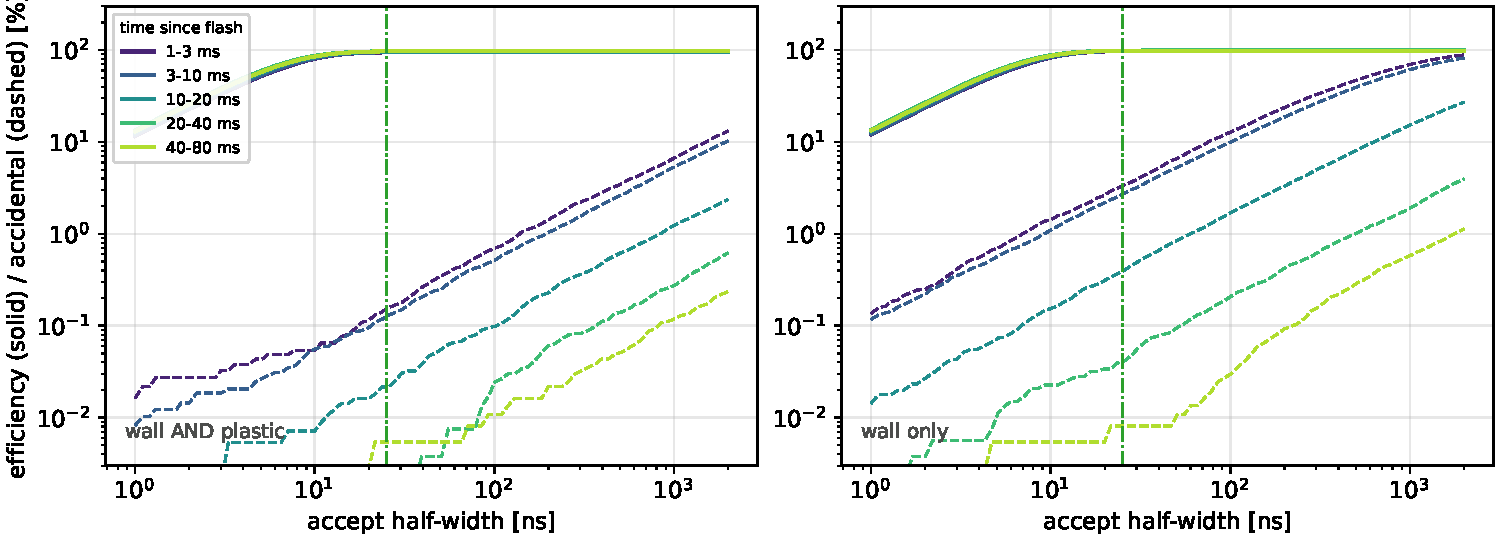
\includegraphics[width=0.97\textwidth]{fig_window_tbins.pdf}
\end{center}
\vspace{-0.5em}
\small
The \ntof{} singles rate falls by $\sim100\times$ from 1--3\,ms to 40--80\,ms, so
the accidental curves are stacked over two decades --- but the \emph{efficiency}
curves lie on top of each other. \hl{One window is right at all times}: the knee
sits at $23.6\ns$ in every time bin and on both legs (28\,ns in the single
hardest bin, wall-only at 1--3\,ms). This is what the per-bunch calibration
buys: without it the knee would move with time since flash, and no single window
could serve the whole spill.
\end{frame}

% ------------------------------------------------------------------
\begin{frame}{The operating point: $\pm25\ns$, one band}
\begin{columns}[T]
\begin{column}{0.52\textwidth}
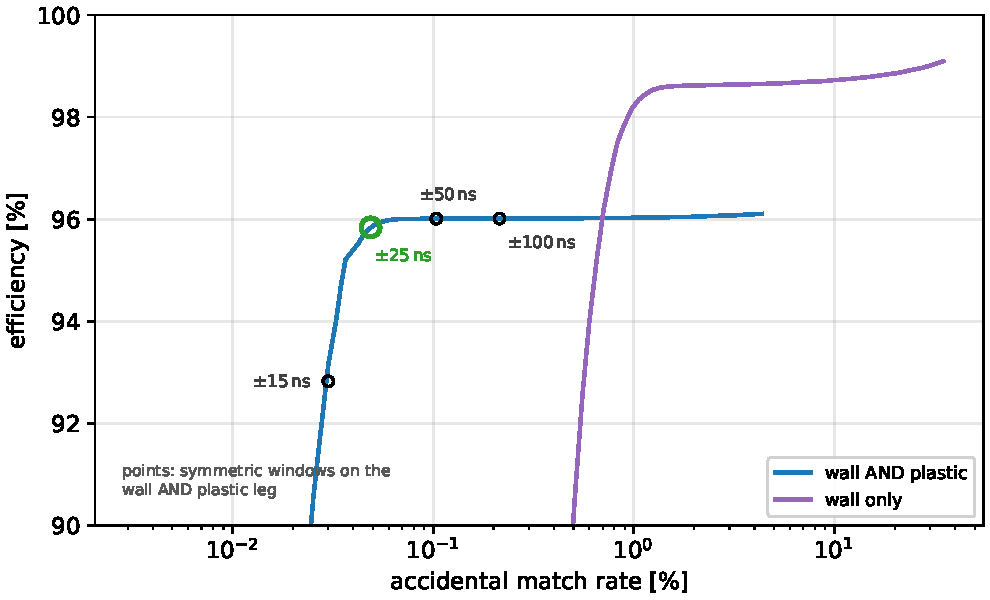
\includegraphics[width=\textwidth]{fig_roc.pdf}
\end{column}
\begin{column}{0.46\textwidth}\small
Criterion: the \emph{tightest} window still within 0.5\,\% (relative) of the
efficiency plateau. It lands at $23.6\ns$ $\Rightarrow$ quote \hl{$\pm25\ns$}.
\vspace{0.4em}

\begin{tabular}{lrrr}
\toprule
wall\,\&\,plastic & eff & accid. & purity\\
\midrule
1--3\,ms   & 94.4\,\% & 0.147\,\% & 99.991\,\%\\
3--10\,ms  & 94.7\,\% & 0.128\,\% & 99.993\,\%\\
10--20\,ms & 95.7\,\% & 0.022\,\% & 99.999\,\%\\
20--40\,ms & 96.8\,\% & 0.002\,\% & 99.9999\,\%\\
40--80\,ms & 96.9\,\% & 0.005\,\% & 99.9998\,\%\\
\midrule
all        & \gd{95.8\,\%} & \gd{0.049\,\%} & 99.998\,\%\\
\bottomrule
\end{tabular}
\vspace{0.4em}

\footnotesize
Going wider is not free and does not pay: $\pm150\ns$ costs $7\times$ the
background for $+0.17$ points of efficiency, and nearly doubles the two-arm
ambiguity ($0.15\to0.28\,\%$). Going tighter is expensive: $\pm15\ns$ already drops
3 points.
\end{column}
\end{columns}
\end{frame}

% ------------------------------------------------------------------
\begin{frame}{What the missing 4\,\% is, and per arm}
\begin{columns}[T]
\begin{column}{0.52\textwidth}
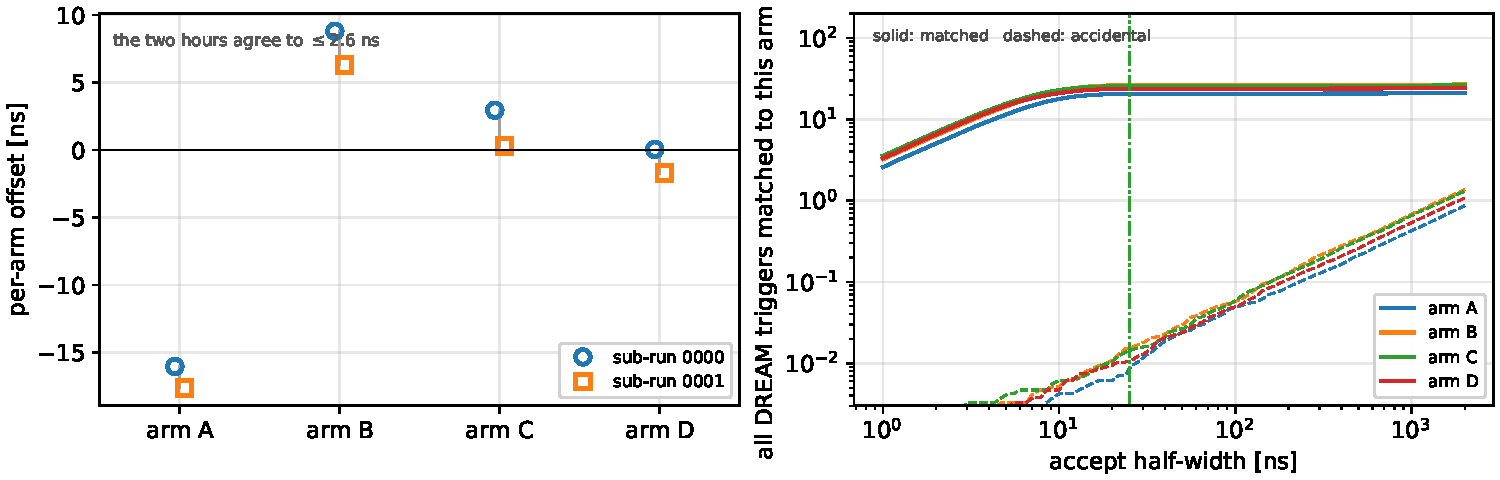
\includegraphics[width=\textwidth]{fig_arms.pdf}
\vspace{-0.2em}

\footnotesize
\textbf{Left:} the per-arm offset is reproducible between the two independent
hours to \gd{$\leq2.6\ns$} --- an instrumental constant of the trigger path, so
it belongs in the calibration. It is \emph{not} a detector misalignment: step 1
sees the four wall flash times within 4\,ns.
\textbf{Right:} each arm takes $\sim$24\,\% of the triggers, and no arm is
anomalous.
\end{column}
\begin{column}{0.46\textwidth}
\small
\begin{tabular}{lr}
\toprule
DREAM triggers                          & 213\,420\\
\midrule
matched, wall only                      & 98.59\,\%\\
matched, wall AND plastic               & 96.00\,\%\\
\midrule
plastic partner $|$ wall matched        & 97.38\,\%\\
plastic leg costs                       & \hl{2.58\,\%}\\
wall leg costs                          & 1.41\,\%\\
\bottomrule
\end{tabular}
\vspace{0.6em}

\footnotesize
(Plateau values --- a window wide enough that the window itself costs nothing, with
the measured accidental rate subtracted.)
\vspace{0.5em}

The plastic leg is the same $\sim$2.6\,\% the \texttt{v12} acceptance test reports,
and it is the one number the reprocessing did not close --- three very different
plastic reconstructions give the same figure, so it is not a pulse-recognition
problem. If it is worth chasing it is the discriminator threshold model, the
channel selection, plastic dead time, or genuine detector inefficiency.
\end{column}
\end{columns}
\end{frame}

% ------------------------------------------------------------------
\begin{frame}{The calibration constants}
\vspace{-0.2em}
\begin{columns}[T]
\begin{column}{0.53\textwidth}
\small
\textbf{Offline, DREAM$\to$\ntof{} time map}\\[0.2em]
\begin{tabular}{llr}
\toprule
$K$    & rate      & $1.103724\times10^{-4}$\\
$T_0$  & offset    & $-253.64\ns$\\
$a_A$  & arm A     & $-16.81\ns$\\
$a_B$  & arm B     & $+7.55\ns$\\
$a_C$  & arm C     & $+1.62\ns$\\
$a_D$  & arm D     & $-0.83\ns$\\
$\delta a_b,\delta k_b$ & per bunch & fitted, $\geq$20 trig.\\
window & accept    & $|r| < 25\ns$, one band\\
\bottomrule
\end{tabular}
\vspace{0.5em}

\textbf{Offline, \ntof{} internal}\\[0.2em]
\begin{tabular}{lr}
\toprule
LIQ, PSS, WAL relative offsets & none needed\\
wall top$-$bottom pairing      & measure per file\\
\texttt{tflash} repair on \texttt{v12} & \textbf{off}\\
\bottomrule
\end{tabular}
\end{column}
\begin{column}{0.45\textwidth}
\small
\textbf{DAQ, as operated in run 224572} (\emph{not} fitted --- read back from
\texttt{n1081b\_config.json} and required to emulate the trigger)\\[0.3em]
\begin{tabular}{lrr}
\toprule
arm & wall thr. & plastic thr.\\
\midrule
A & 25\,mV & 118\,mV\\
B & 35\,mV & 139\,mV\\
C & 34\,mV & 157\,mV\\
D & 36\,mV & 134\,mV\\
\bottomrule
\end{tabular}
\vspace{0.7em}

\footnotesize
\hl{What transfers and what does not.} The DAQ thresholds are hardware state:
valid until someone turns a knob. The \ntof{}-internal alignment is a property
of the \emph{processing} and must be re-measured per reprocessing. $K$, $T_0$
and the per-arm offsets are properties of the pair (DREAM run,
\ntof{} processing) --- \textbf{re-fit them per run}; the per-bunch term is by
construction per bunch and is always re-fitted.
\vspace{0.4em}

Exported to \texttt{nTof\_x17\_DAQ/calibrations/dream\_ntof/}.
\end{column}
\end{columns}
\end{frame}

% ------------------------------------------------------------------
\begin{frame}{Summary, and what it unlocks}
\begin{columns}[T]
\begin{column}{0.52\textwidth}
\textbf{The method}
\begin{enumerate}\setlength\itemsep{0.2em}
  \item Align \ntof{} to itself against the beam pickup; confirm on late
        coincidences. No offsets turn out to be needed \emph{on v12} --- but
        check, do not assume.
  \item Rebuild the N1081B sector SINGLES from the hit trees, with the
        thresholds the run actually held.
  \item Fit the global time map ($K$, $T_0$, per arm) on the whole run.
  \item Fit $(\delta a_b,\delta k_b)$ per bunch on its own matched triggers.
  \item Accept $|r|<25\ns$, single band.
\end{enumerate}
\vspace{0.3em}
\footnotesize
Reproducible end to end from \texttt{ntof\_dream\_merge/match\_study/};
constants and the per-run recipe in
\texttt{ntof\_dream\_merge/DREAM\_NTOF\_CALIBRATION.md}.
\end{column}
\begin{column}{0.46\textwidth}
\textbf{Why it matters for the Micromegas}
\begin{itemize}\setlength\itemsep{0.3em}
  \item The MM cross-check keys on \emph{which arm} fired. At $\pm25\ns$ the
        two-arm ambiguity is \gd{0.15\,\%} and the accidental contamination of
        the matched sample is \gd{0.049\,\%} --- both directly limit how sharply
        an arm-vs-chamber correlation can be measured.
  \item A \gd{$6\ns$} match residual means the \ntof{} wall time can be used as
        an \emph{absolute} time reference for the MM drift window. At the
        30--40\,ns level that was not possible.
  \item The liquid leg is already on the wall time base to under a nanosecond,
        so it can join without further calibration.
\end{itemize}
\end{column}
\end{columns}
\end{frame}

\end{document}
